% \documentclass{article}
\documentclass[preprint,12pt]{elsarticle}

%% PACKAGES
\usepackage[margin=1.5cm,includefoot]{geometry}
\usepackage{setspace}

% uploading packages
\usepackage{graphicx}
\usepackage{amssymb}
\usepackage{textcomp} % https://latex.org/forum/viewtopic.php?f=4&t=3364#p13124, https://tex.stackexchange.com/questions/165115
\usepackage{gensymb}
\usepackage{lineno}
\usepackage{mathtools}
\usepackage[title]{appendix}
\usepackage[separate-uncertainty=true]{siunitx}
% \usepackage{xr-hyper} %needs to  be before hyperref
\usepackage[colorlinks]{hyperref}
\PassOptionsToPackage{hyphens}{url}\usepackage{hyperref} %allow URLs to break across lines
\usepackage[nameinlink,capitalise]{cleveref} %needs to appear after hyperref, https://tex.stackexchange.com/questions/396728/my-equations-referencing-not-working
\Crefname{figure}{Figure}{Figures} %needs to appear after hyperref and cleveref
\crefname{appsec}{Appendix}{Appendices}
\newcommand\crefrangeconjunction{--} % modify the reference style
\usepackage{mathrsfs}
\usepackage{chemformula} %alternative: \usepackage{mhchem}, both for chemical formulas
\usepackage{url}
\usepackage{enumitem}
\usepackage{tabulary}
\usepackage{caption}
\usepackage{subcaption}
\usepackage{multirow}
\usepackage{makecell} % https://tex.stackexchange.com/questions/2441/how-to-add-a-forced-line-break-inside-a-table-cell
\graphicspath{{figures/}} %Setting the graphicspath
% ---------to deal with the double quotes----------- 
\usepackage [english]{babel}
\usepackage [autostyle, english = american]{csquotes}
\MakeOuterQuote{"}
%alternatively can use `` '' format for double quotes
\usepackage{matlab-prettifier}
\newcommand{\matlab}[1]{\mbox{\lstinline[style=Matlab-editor]{#1}}}
\usepackage{booktabs}
\setlength{\abovetopsep}{1ex}
\usepackage[shortcuts,abbreviations,automake]{glossaries-extra}

\usepackage{nameref,zref-xr}
\zxrsetup{toltxlabel}

% remove the "Preprint submitted to Elsevier" footer on the first page
\makeatletter
\def\ps@pprintTitle{%
   \let\@oddhead\@empty
   \let\@evenhead\@empty
   \def\@oddfoot{\reset@font\hfil\thepage\hfil}
   \let\@evenfoot\@oddfoot
}
\makeatother

%% Cross referencing with the xr package in Overleaf (https://www.overleaf.com/learn/how-to/Cross_referencing_with_the_xr_package_in_Overleaf)
\makeatletter
\newcommand*{\addFileDependency}[1]{% argument=file name and extension
  \typeout{(#1)}
  \@addtofilelist{#1}
  \IfFileExists{#1}{}{\typeout{No file #1.}}
}
\makeatother
\newcommand*{\myexternaldocument}[1]{%
    \externaldocument{#1}%
    \addFileDependency{#1.tex}%
    \addFileDependency{#1.aux}%
}

\glssetcategoryattribute{abbreviation}{indexonlyfirst}{true}
\glssetcategoryattribute{abbreviation}{nohyper}{true}
\newabbreviation{ml}{ML}{machine learning}


\makeglossaries

%Import the natbib package and sets a bibliography  and citation styles
% \usepackage{natbib}
%https://www.overleaf.com/learn/latex/natbib_citation_styles

\title{Cartesian closed categories and the price of eggs}
\author{Jane Doe}
\date{September 1994}
\begin{document}
   \maketitle
   Hello world!

We present breakdown time data for various research activities in \cref{tab:breakdown}.
% Please add the following required packages to your document preamble:
% \usepackage{booktabs}
\begin{table}[h!]
\centering
\caption{Example of breakdown of time spent.}
\label{tab:breakdown}
\begin{tabular}{@{}lll@{}}
\toprule
Task                             & Time Spent (minutes) & Time We Wish We Spent (minutes) \\ \midrule
Fiddling with equations          & 120                  & 5                               \\
Correcting reference order       & 60                   & 0                               \\
Looking for "that one" reference & 90                   & 1                               \\
Copy-pasting figures             & 20                   & 0                               \\
Rerunning all data               & 180                  & 20                              \\
Fixing reference meta-data       & 60                   & 0                               \\
Actually doing research          & 900                  & 1500                            \\ \bottomrule
\end{tabular}
\end{table}

An example of an equation is Fick's second law (\cref{eq:fick-second}).
\begin{equation} \label{eq:fick-second}
    \frac{\partial \varphi}{\partial t}=D \frac{\partial^{2} \varphi}{\partial x^{2}}
\end{equation}





Once we've defined abbreviations in \texttt{abbrev.tex}, we can call those abbreviations using the \texttt{gls} command. In the case of ``machine learning'', the first usage of \texttt{gls} will give the full form as in \gls{ml}. The next usage of \texttt{gls} will give the abbreviated version as in \gls{ml}.

After we've included the bibliography file in the \texttt{bibliography} command, we can start citing articles using the \texttt{natbib} \texttt{cite} and \texttt{citet} commands, as in the following example:

\citet{wangMachineLearningMaterials2020a} emphasized the need for reproducible methods and benchmarking. Another work further emphasized the importance of these topics \cite{barnardBestPracticeLeads2020}.

Typesetting equations in Mathematica can be very effective. Here is an example of a teaching figure: \\ %For example, we have the following equation which demonstrates a possible representation of a crystal structure using Gaussian encodings of distances, angles, areas, and volumes defined by the crystal's atomic positions: \\

\resizebox{.9\hsize}{!}{\begin{equation}
    \begin{array}{cccc}
     \overbrace{\left(
    \begin{array}{c}
     \text{Distances} \\
     \text{Angles} \\
     \text{Area} \\
     \text{Volume} \\
    \end{array}
    \right)}^{\text{Features}} & \overbrace{\left(
    \begin{array}{c}
     0.1\text{\AA} \\
     0\text{rad} \\
     0\text{\AA}^2 \\
     0\text{\AA}^3 \\
    \end{array}
    \right)}^{\text{Lower Bound}} & \overbrace{\left(
    \begin{array}{ccccccccccccc}
     0 & 0.1 & 0.3 & 0.1 & 0 & 0 & 0.2 & 0.4 & 0.2 & 0 & 0 & \ldots  & 0 \\
     0 & 0.1 & 0.2 & 0.4 & 0.2 & 0.1 & 0 & 0 & 0 & 0 & 0 & \ldots  & 0.2 \\
     0 & 0 & 0 & 0.3 & 0.6 & 0.3 & 0 & 0 & 0 & 0.1 & 0.2 & \ldots  & 0 \\
     0 & 0 & 0 & 0 & 0 & 0.4 & 0.6 & 0.4 & 0 & 0 & 0 & \ldots  & 0.1 \\
    \end{array}
    \right)}^{\text{Gaussian Encoding}} & \overbrace{\left(
    \begin{array}{c}
     15\text{\AA} \\
     \pi \text{rad} \\
     225\text{\AA}^2 \\
     3375\text{\AA}^3 \\
    \end{array}
    \right)}^{\text{Upper Bound}} \\
    \end{array}
\end{equation}}

Figures and captions can be generated programmatically. See \cref{} for example :

\begin{figure}[h]
	\centering
	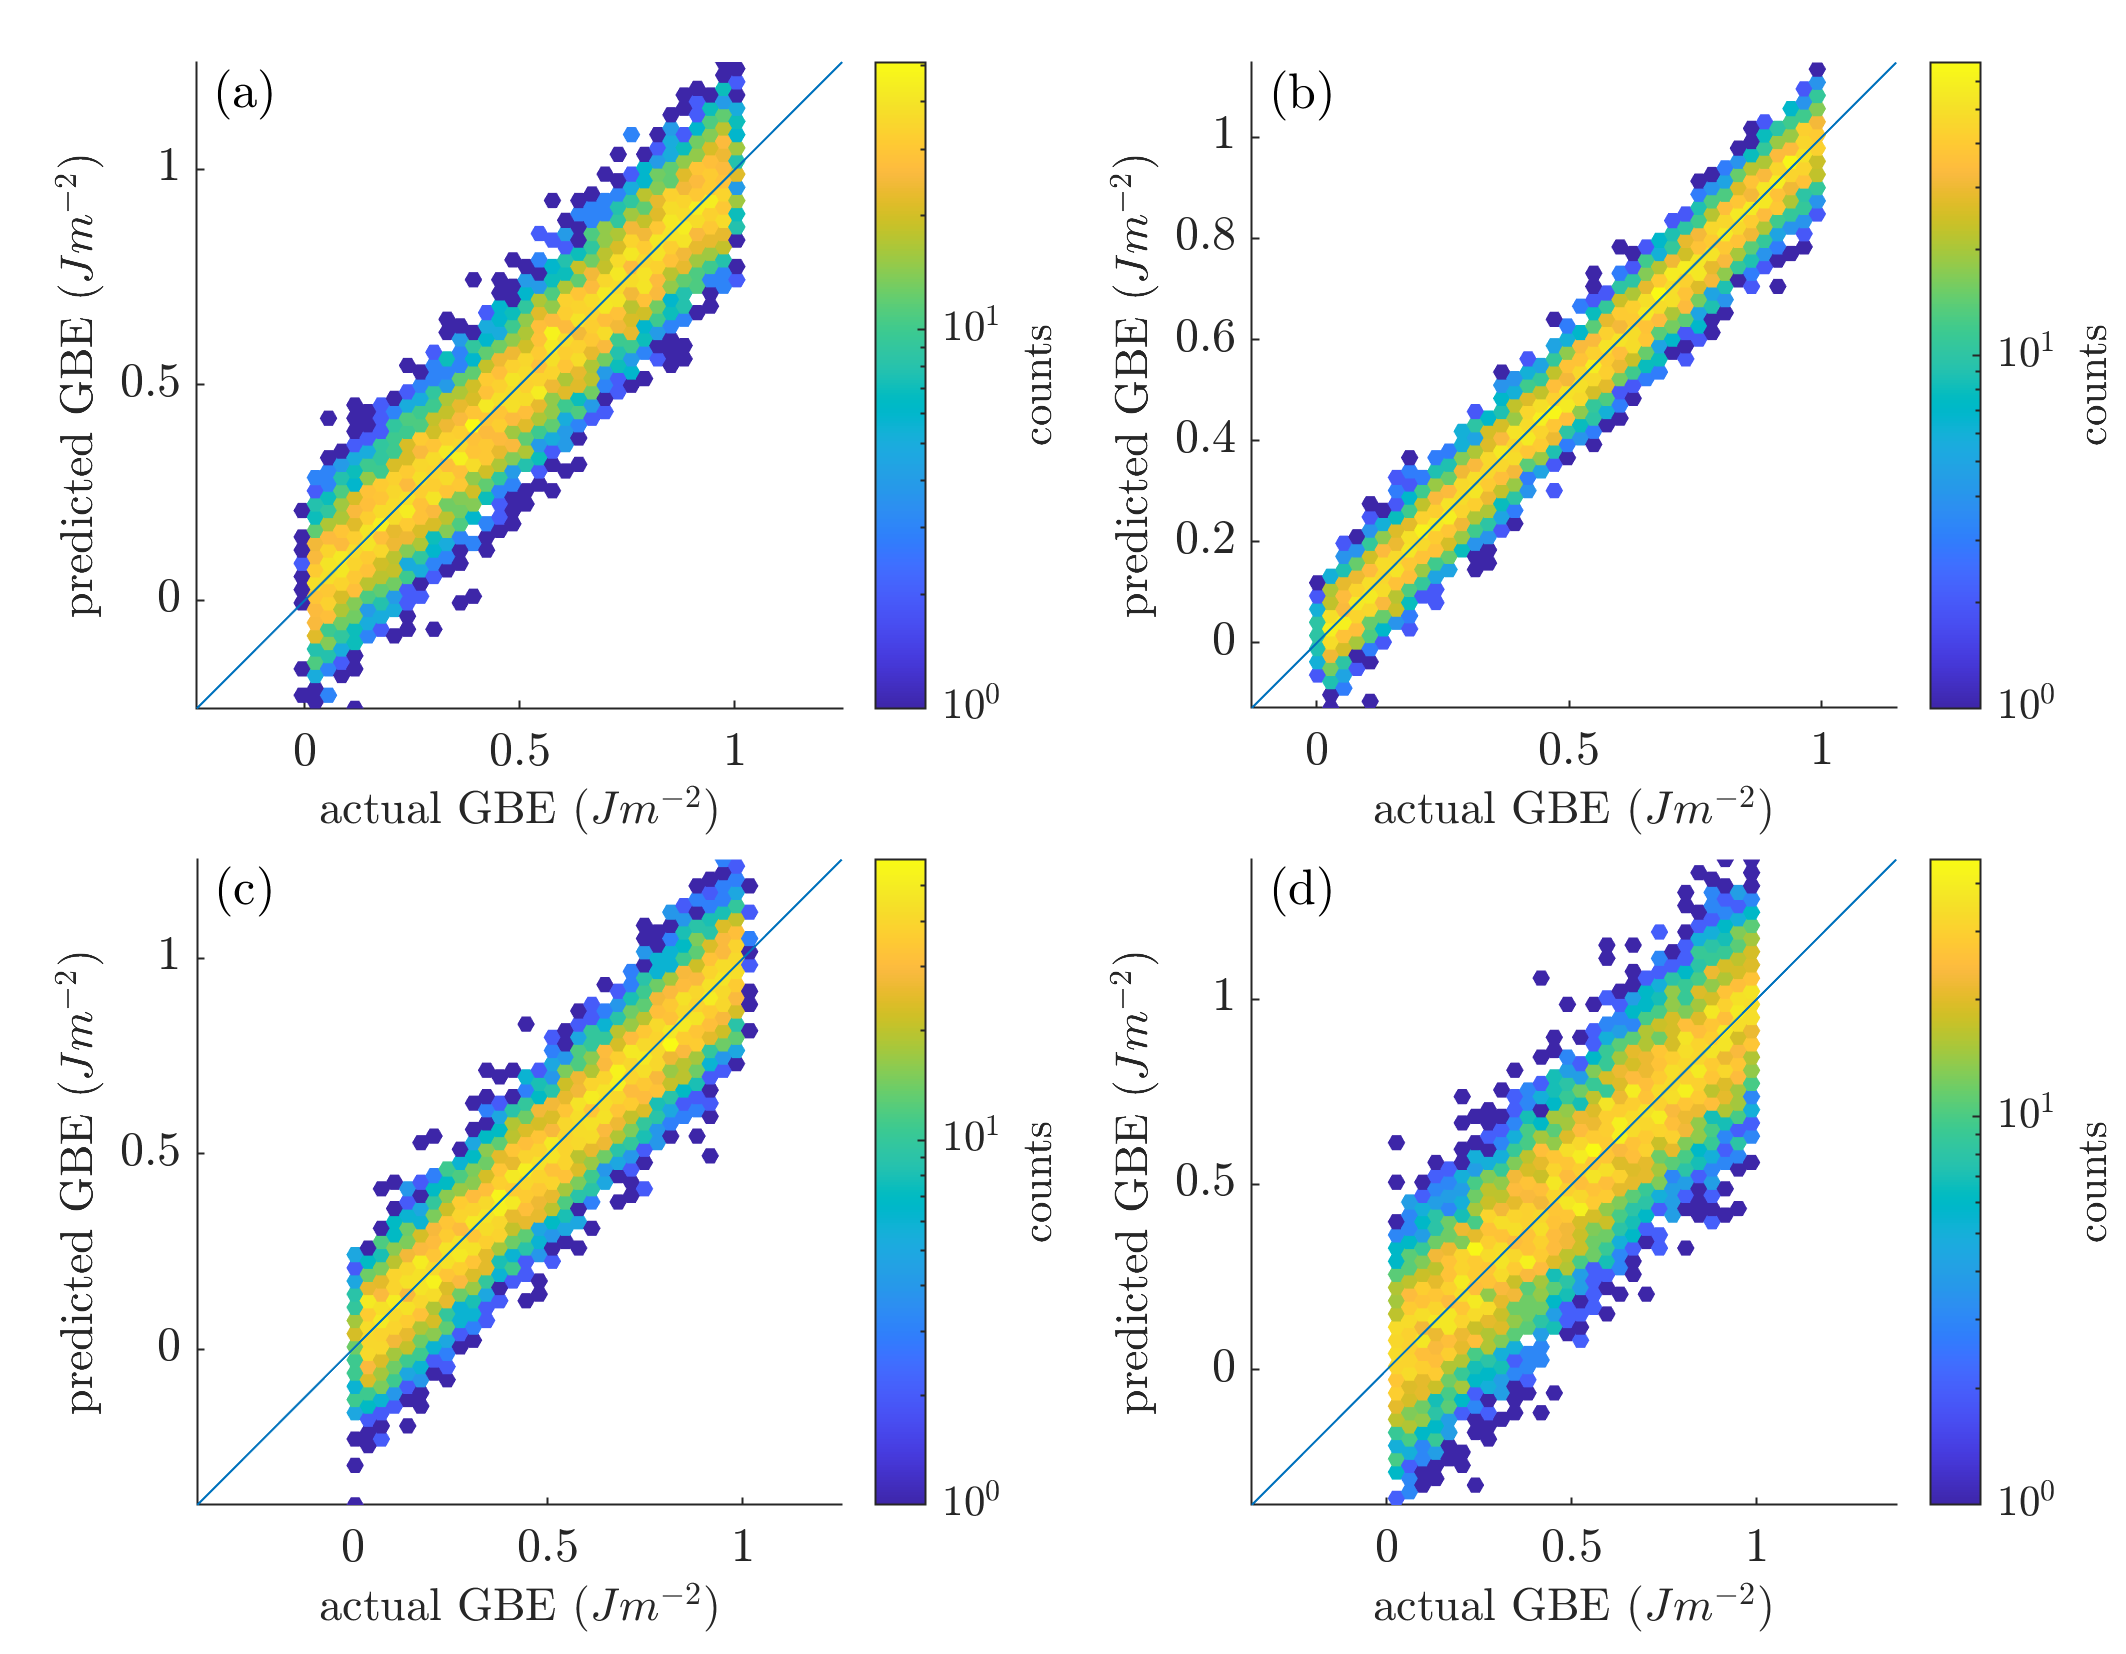
\includegraphics[scale=1]{figures/multi-parity.png}
	\label{fig:parity-test}
	\caption{Parity plots with \glspl{rmse} of (a) 0.098456, (b) 0.050737, (c) 0.099079,  and (d) 0.14963 \SI{}{\J\per\square\m}.}
\end{figure}

\printglossaries

\bibliographystyle{elsarticle-num-names}
\bibliography{auto-paper}

\end{document}

